%% 
%%	This is file 'beamer_sample.tex'
%%	according to an MPIDR's PowerPoint template (?)
%%	
%%	by Eric Naujoks
%%
%%	Problems, bugs and comments to 
%%	naujoks@demogr.mpg.de
%%

%%%%%%%%%%%%%%%%%%%%%%%%%%%%%%%%%%
%%	Praelegomena								%%
%%%%%%%%%%%%%%%%%%%%%%%%%%%%%%%%%%
%%	- Make sure that you use utf8-encoding for all your .tex-files!!! (TeXnicCenter since version 2.0)
%%	- TeXnicCenter update: MPIDR intranet > Hard- & Sortfware > Software > Script and text editors > TeXnicCenter

\documentclass[20pt,usenames,dvipsnames]{beamer}

\usepackage[ngerman,english]{babel}
\usepackage{tikz}
\usepackage[normalem]{ulem}
\geometry{paperwidth=10in, paperheight=7.5in}
\usepackage{animate}

\usepackage[utf8]{inputenc}

\usepackage[mpidr]{./mpidr/beamerthemeMPIDR}
%\usefonttheme{serif}
%\newcolumntype{C}[1]{>{\centering\let\newline\\\arraybackslash\hspace{0pt}}m{#1}}
%\newcommand*{\QEDA}{\hfill\ensuremath{\blacksquare}}
%% Declaring title and author
%	the institute's logo
%\renewcommand{\mylogo}{\includegraphics[width=4.7in]{mpidr_logo_colour_en}}
\usepackage{color}
\definecolor{mygray}{rgb}{0.8,0.8,0.8}
\definecolor{yellow}{rgb}{1,1,0}

\defbeamertemplate{description item}{align left}{\insertdescriptionitem\hfill}
%%	should be the very last package to be loaded
\usepackage{hyperref}

%%%%%%%%%%%%%%%%%%%%%%%%%%%%%%%%%%
%%	Beginning of the document		%%
%%%%%%%%%%%%%%%%%%%%%%%%%%%%%%%%%%
\begin{document}

%%	titlepage - fixed frame:
%%	========================

% \begin{frame}
% 	\titlepage
% \end{frame}
\begin{frame}[plain]
	%\titlepage
	\vspace{-3cm}
 \centerline{\includegraphics[scale=.165]{beamerstrip3.png}}

	
	\huge
	\vspace{1em}
	
	Healthy lives: Delayed onset, improved recovery, or mortality
change?\\
	\vspace{1em}
	\large 
	Tim Riffe, Neil Mehta, Daniel Schneider, Mikko Myrskyl\"a 
\end{frame}
%-------------------
\begin{frame}[plain]
\Large
\begin{block}{Objective}
How much of the change in life expectancy at age 50 $e(50)$ is due to changes in mortality versus changes in disability transitions?
\end{block}
\end{frame}
%-------------------
\begin{frame}[plain]
\Large
\begin{block}{Data \& Methods}
\begin{itemize}
\item HRS RAND version P. 
\item Transition probabilities: mlogit with age and time splines (3 knots).
\item Controls for race/eth (4) and education (3). 
\item 3-state Markov matrix models centered on years 1996, 2006, and 2014. 
\item Trend decomposition using Horiuchi et. al. (2007) method.
\end{itemize}
\end{block}
\end{frame}

\begin{frame}[plain]
\Large
\begin{center}
State space
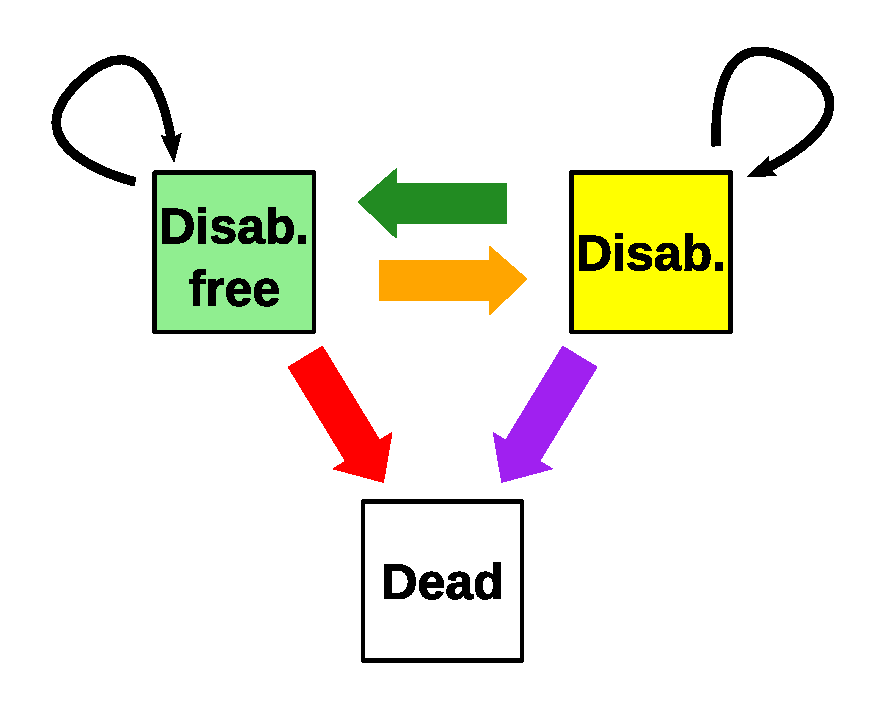
\includegraphics[height=\textheight, keepaspectratio]{Figures/StateSpace.pdf}
\end{center}
\end{frame}

\begin{frame}[plain]
\vspace{-1em}
\begin{center}
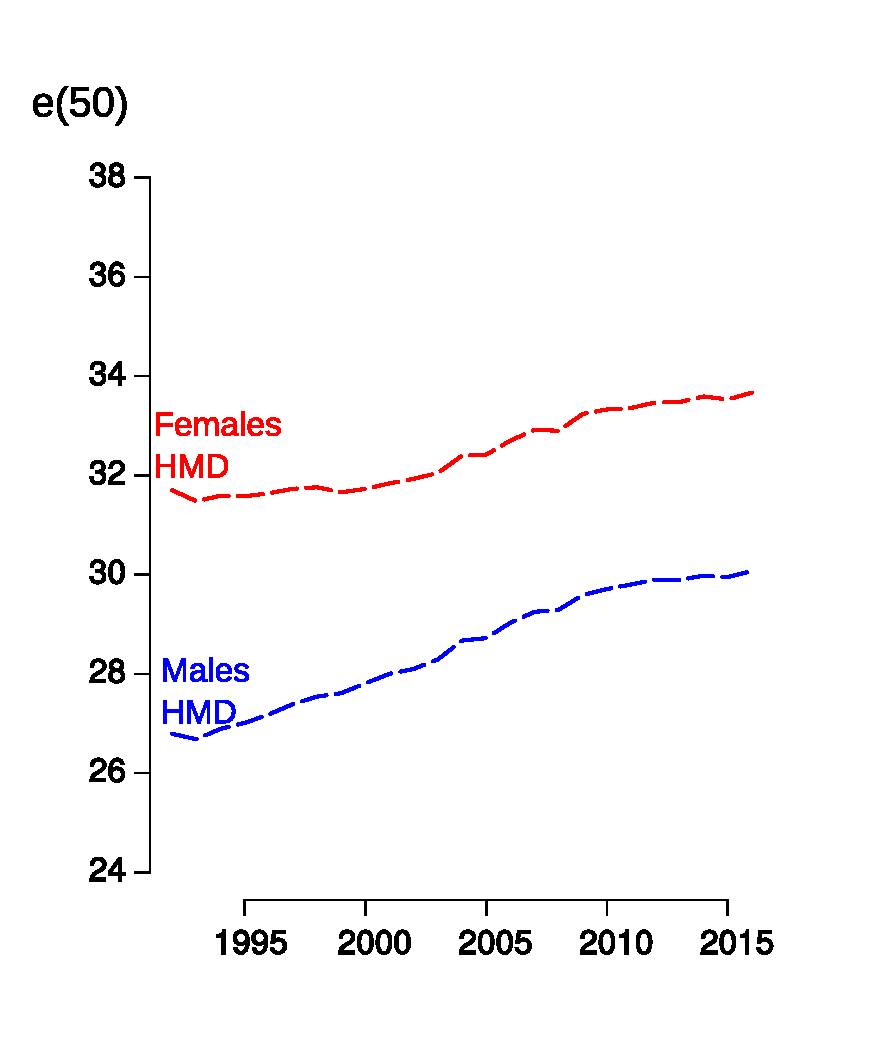
\includegraphics[height=20cm, keepaspectratio]{Figures/e50_0.pdf}
\end{center}
\end{frame}
\begin{frame}[plain]
\vspace{-1em}
\begin{center}
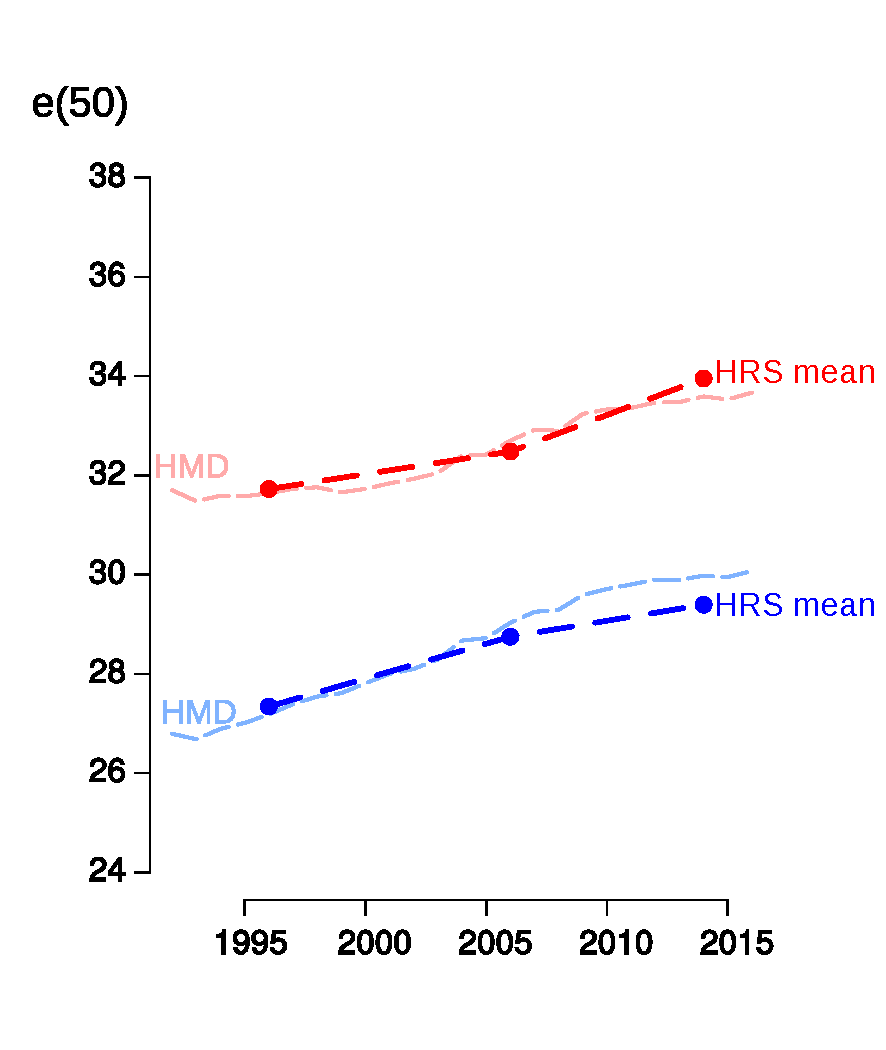
\includegraphics[height=20cm, keepaspectratio]{Figures/e50_1.pdf}
\end{center}
\end{frame}
\begin{frame}[plain]
\vspace{-1em}
\begin{center}
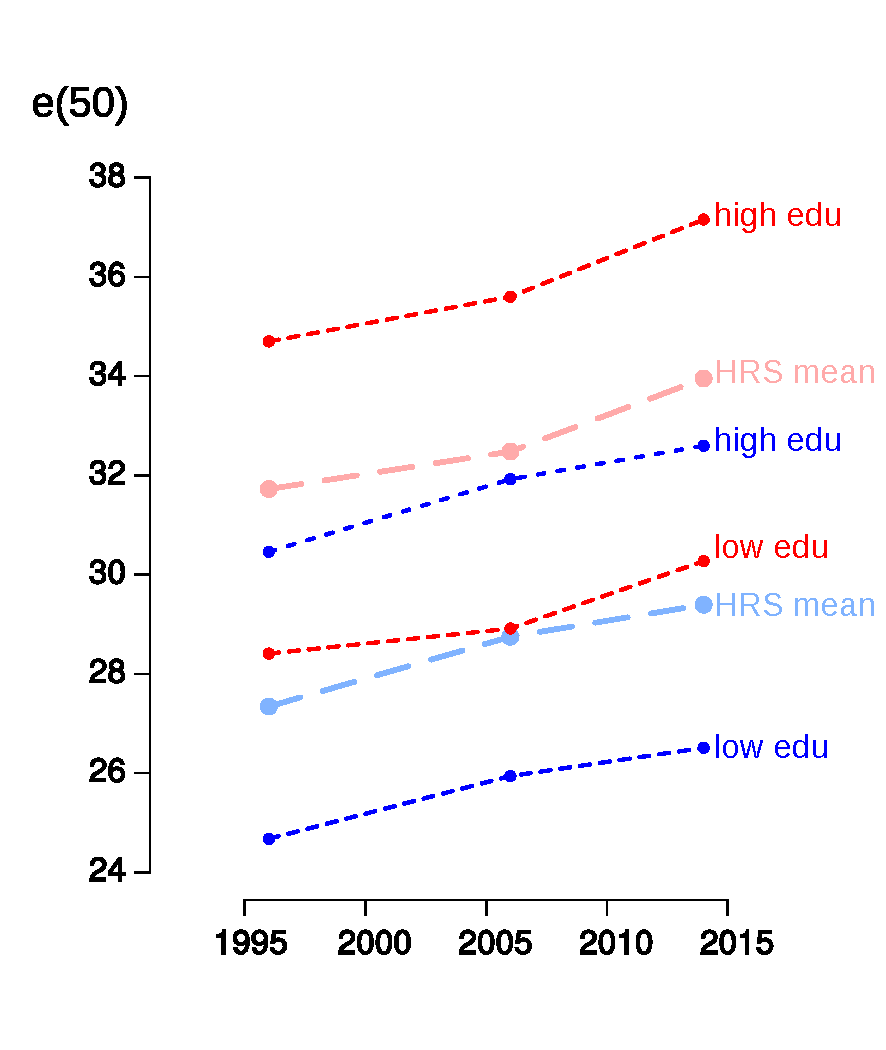
\includegraphics[height=20cm, keepaspectratio]{Figures/e50_2.pdf}
\end{center}
\end{frame}
\begin{frame}[plain]
\vspace{-1em}
\begin{center}
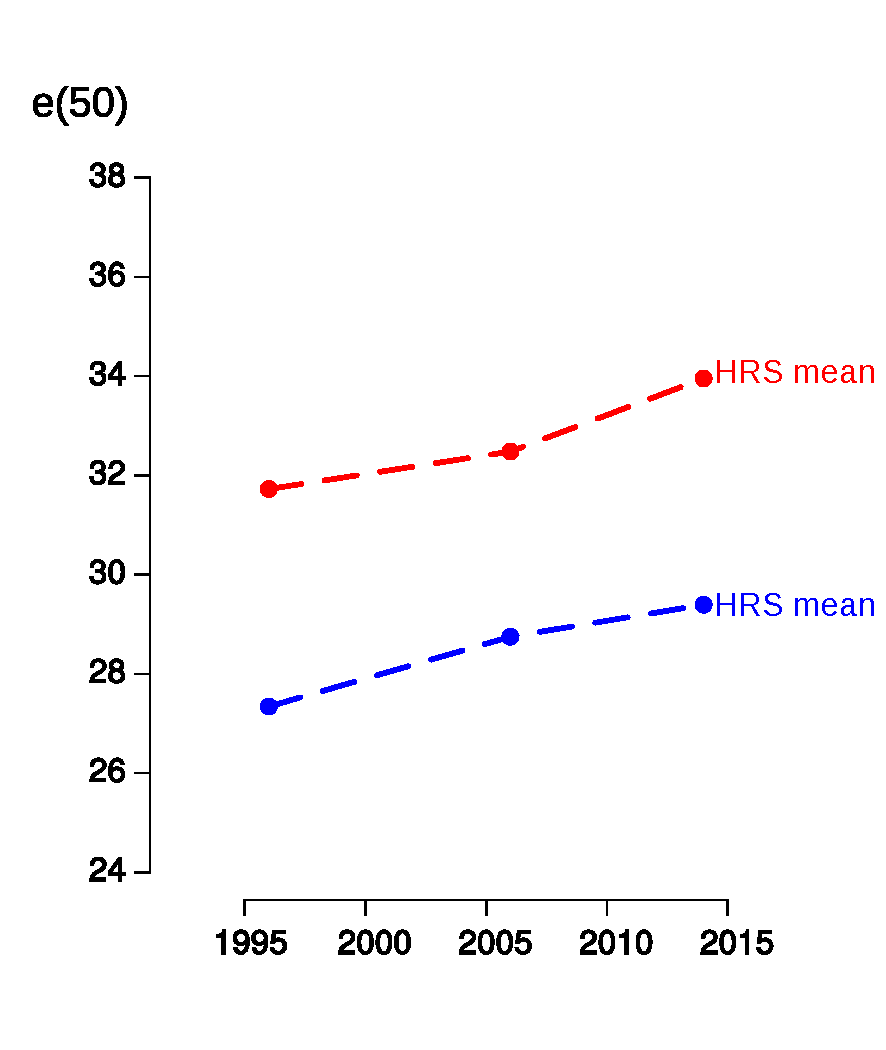
\includegraphics[height=20cm, keepaspectratio]{Figures/e50_3.pdf}
\end{center}
\end{frame}
\begin{frame}[plain]
\vspace{-1em}
\begin{center}
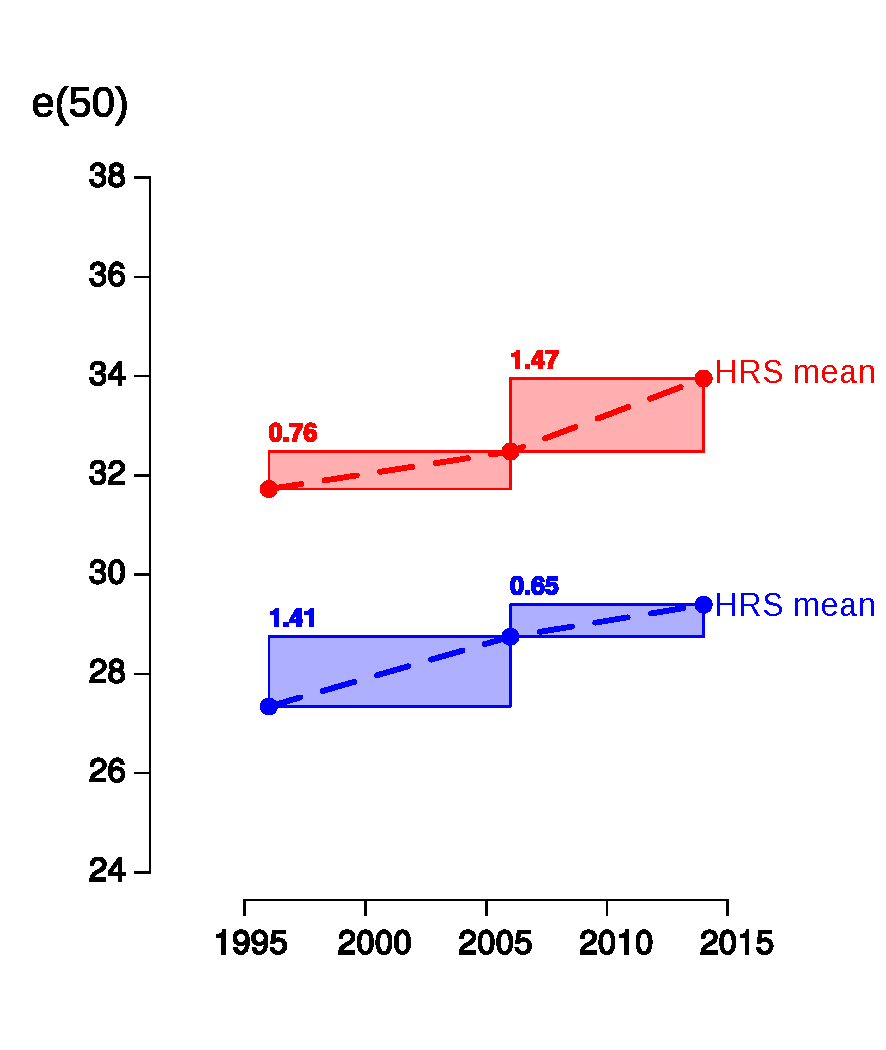
\includegraphics[height=20cm, keepaspectratio]{Figures/e50_4.pdf}
\end{center}
\end{frame}

%\begin{overlayarea}{\textwidth}{.8\textheight}
%\begin{center}
%\only<1>{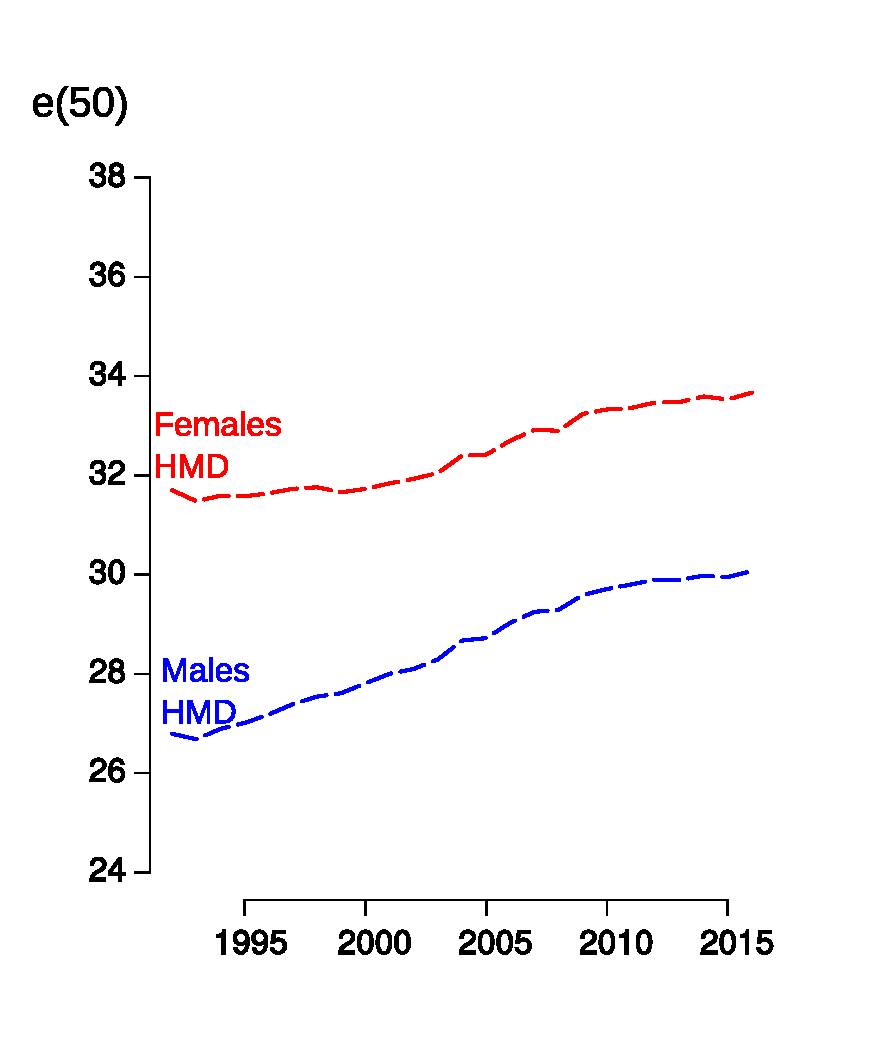
\includegraphics[height=\textheight, keepaspectratio]{Figures/e50_0.pdf}}
%\only<2>{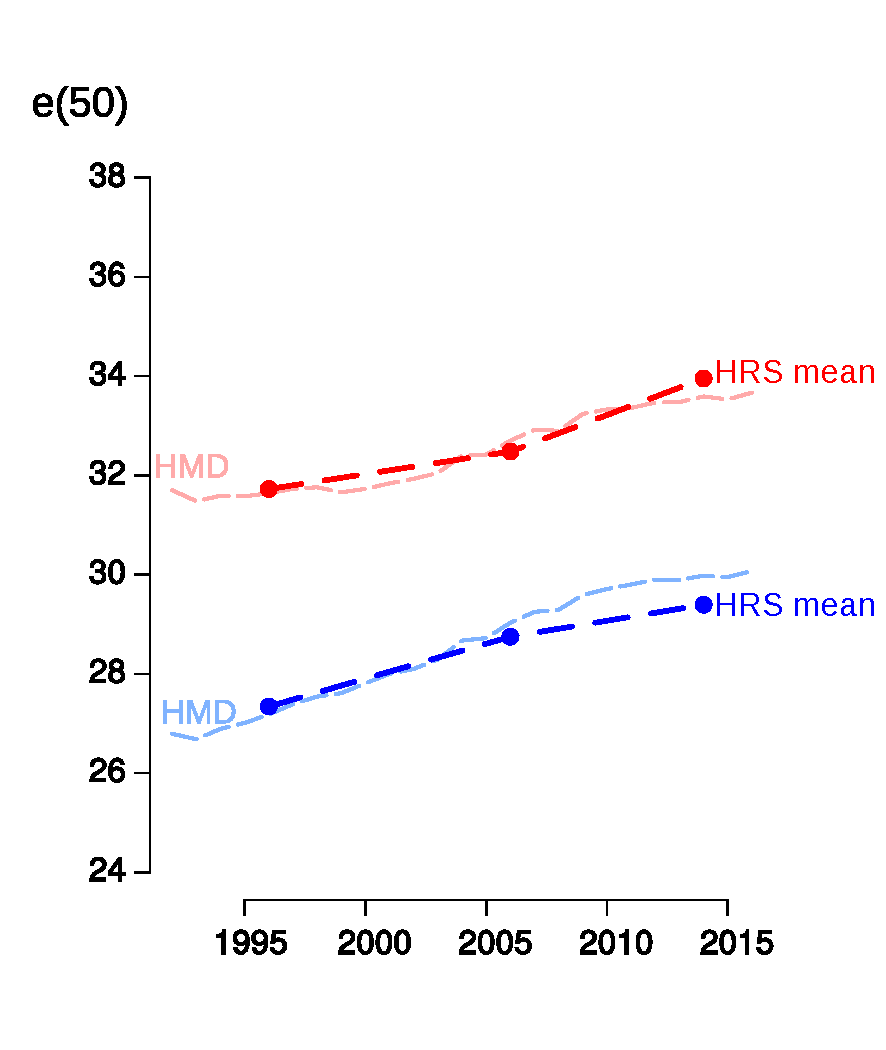
\includegraphics[height=\textheight, keepaspectratio]{Figures/e50_1.pdf}}
%\only<3>{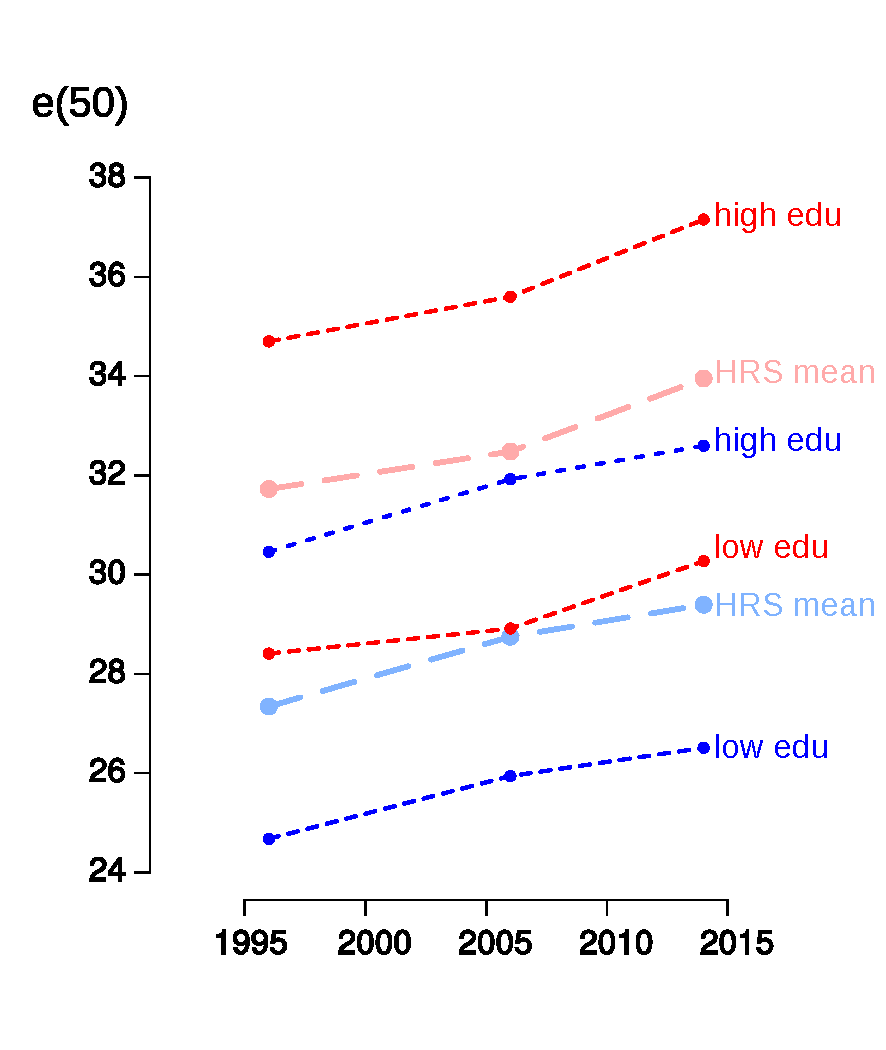
\includegraphics[height=\textheight, keepaspectratio]{Figures/e50_2.pdf}}
%\only<4>{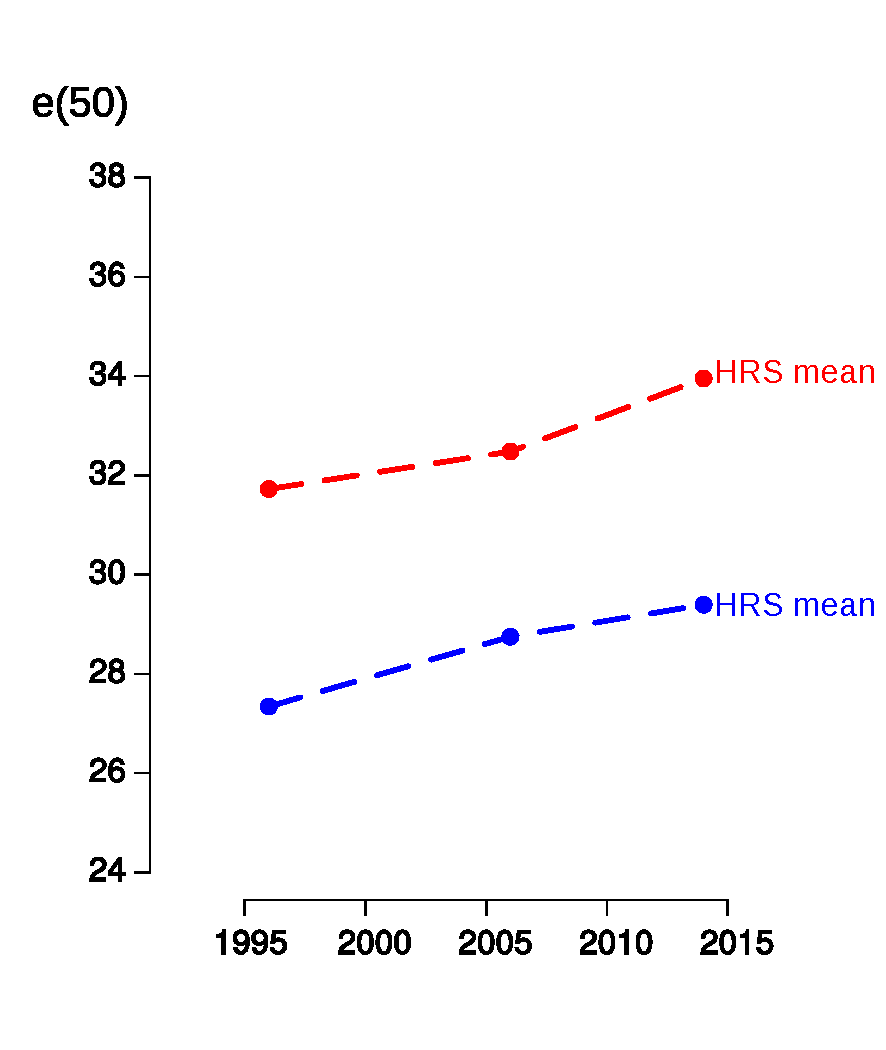
\includegraphics[height=\textheight, keepaspectratio]{Figures/e50_3.pdf}}
%\only<5>{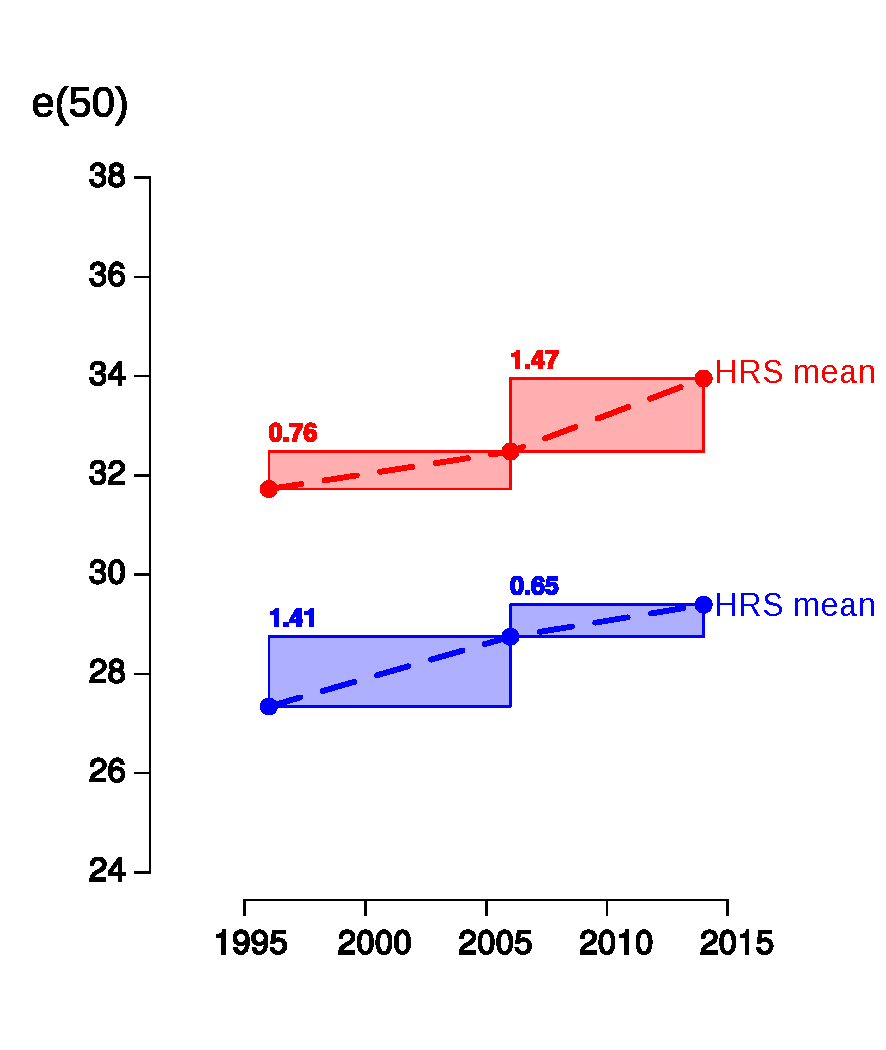
\includegraphics[height=\textheight, keepaspectratio]{Figures/e50_4.pdf}}
%\end{center}
%\end{overlayarea}
%\end{frame}
%

\begin{frame}[plain]
\Large\begin{center}
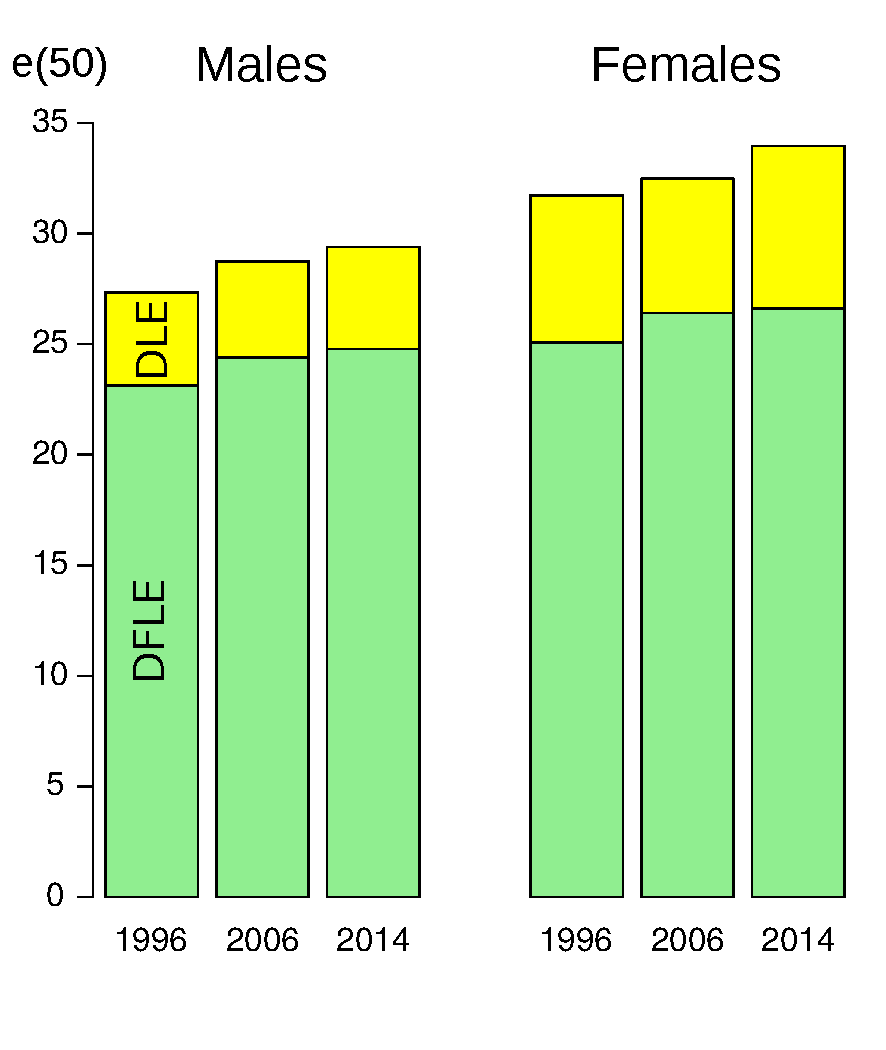
\includegraphics[height=\textheight, keepaspectratio]{Figures/lemf_ink.pdf}
\end{center}
\end{frame}


%\begin{frame}[plain]
%\Large
%\vspace{1em}
%\begin{overlayarea}{\textwidth}{\textheight}
%\begin{center}
%\only<1>{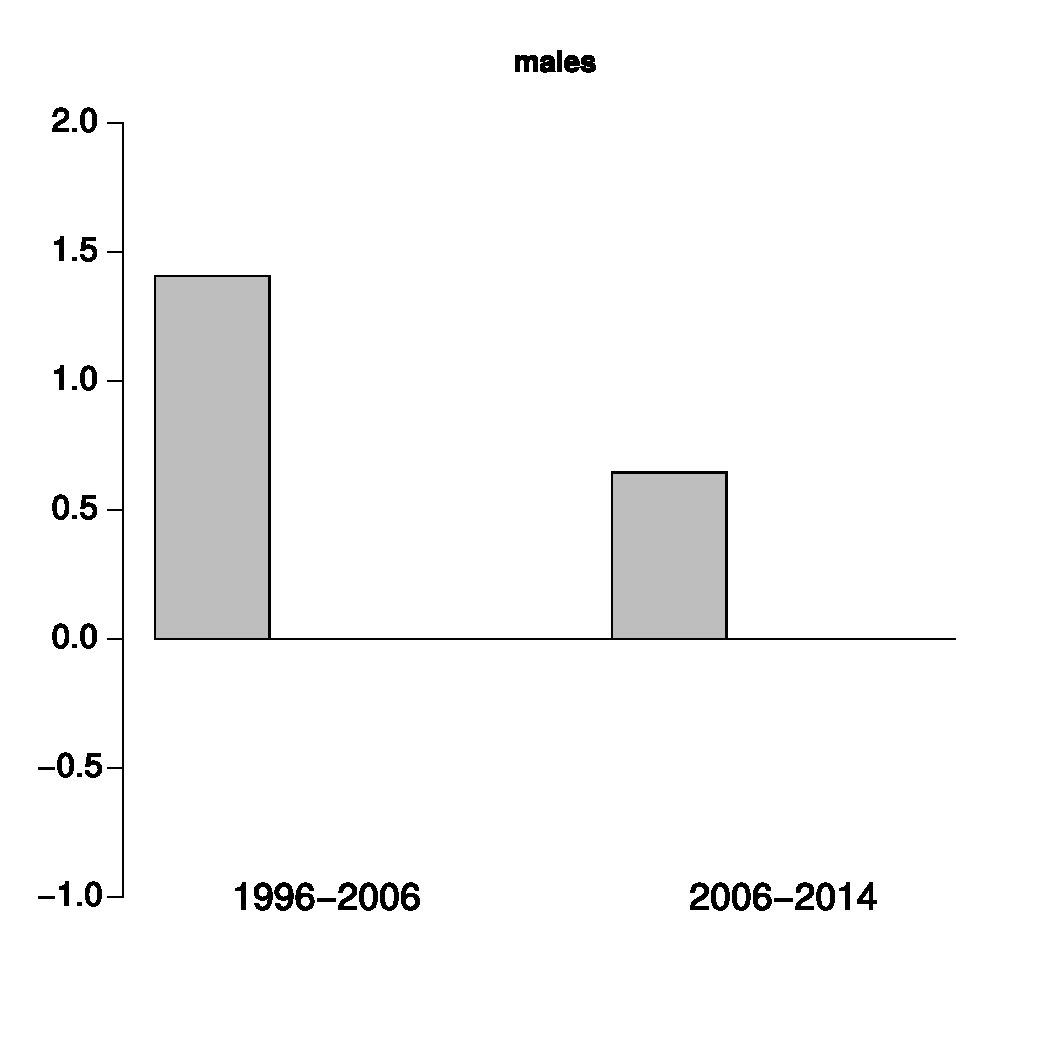
\includegraphics[height=\textheight, keepaspectratio]{Figures/MalesDecAllEdu1.pdf}}
%\only<2>{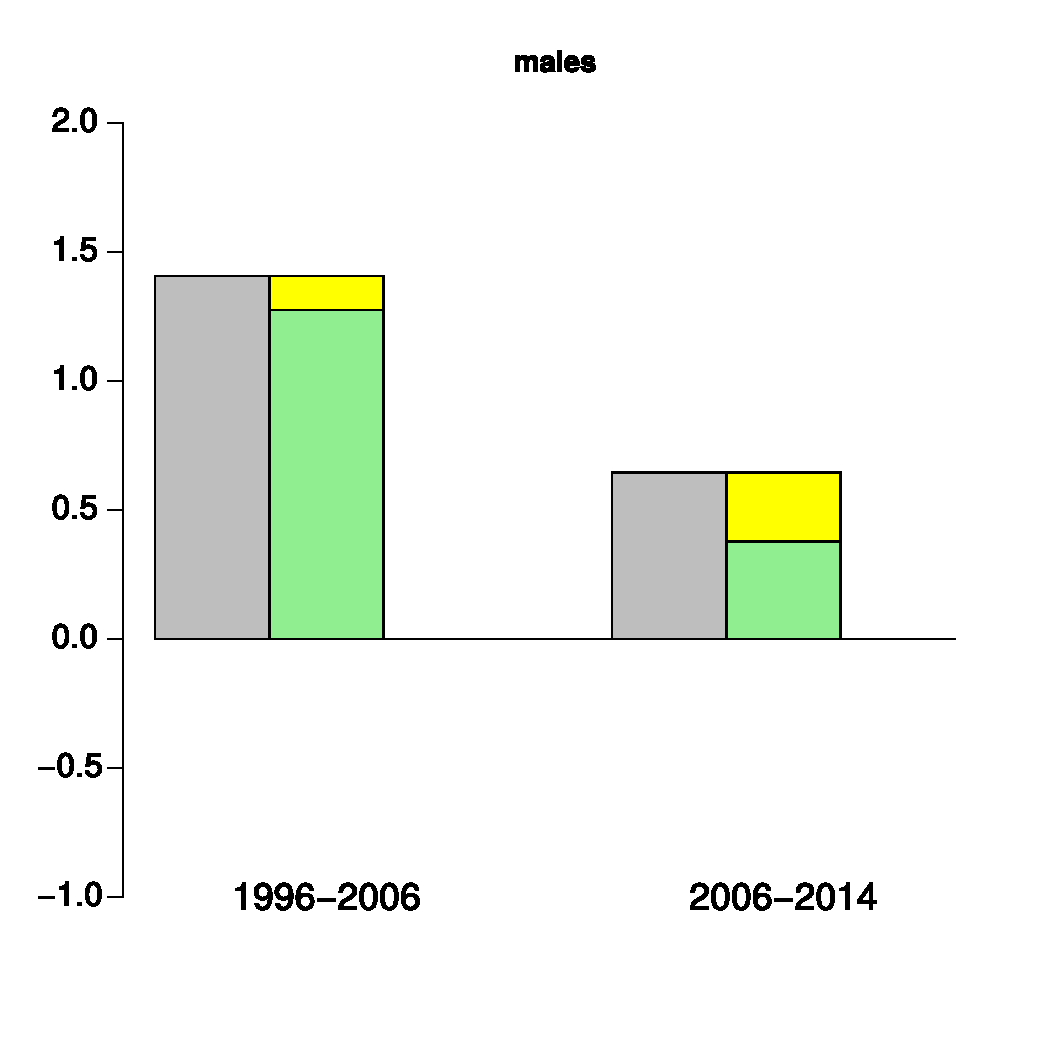
\includegraphics[height=\textheight, keepaspectratio]{Figures/MalesDecAllEdu2.pdf}}
%\only<3>{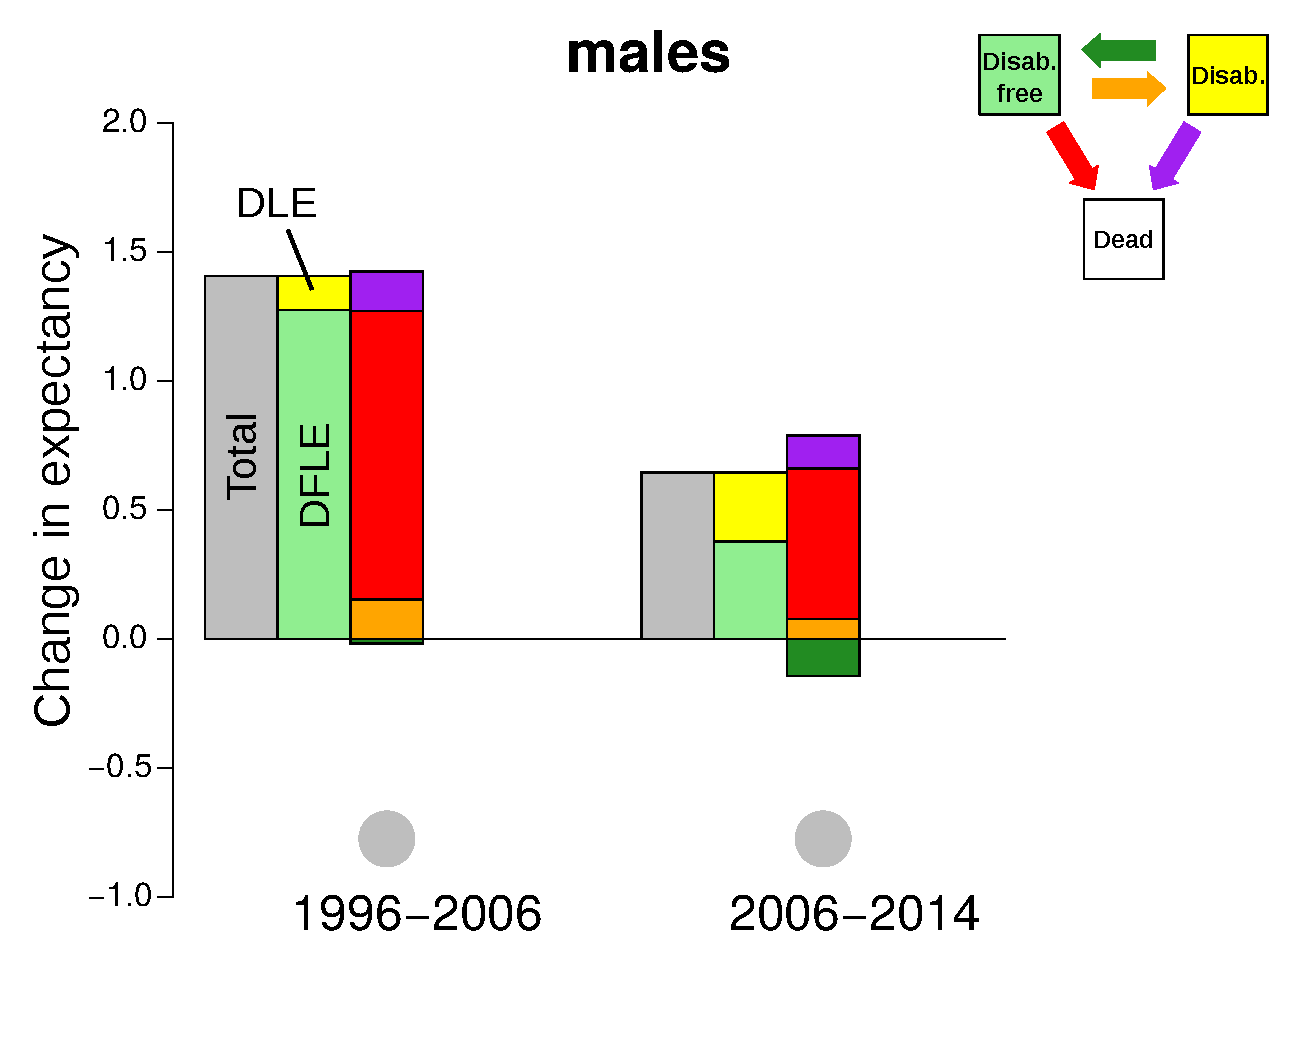
\includegraphics[height=\textheight, keepaspectratio]{Figures/MalesDecAllEdu3.pdf}}
%\only<4>{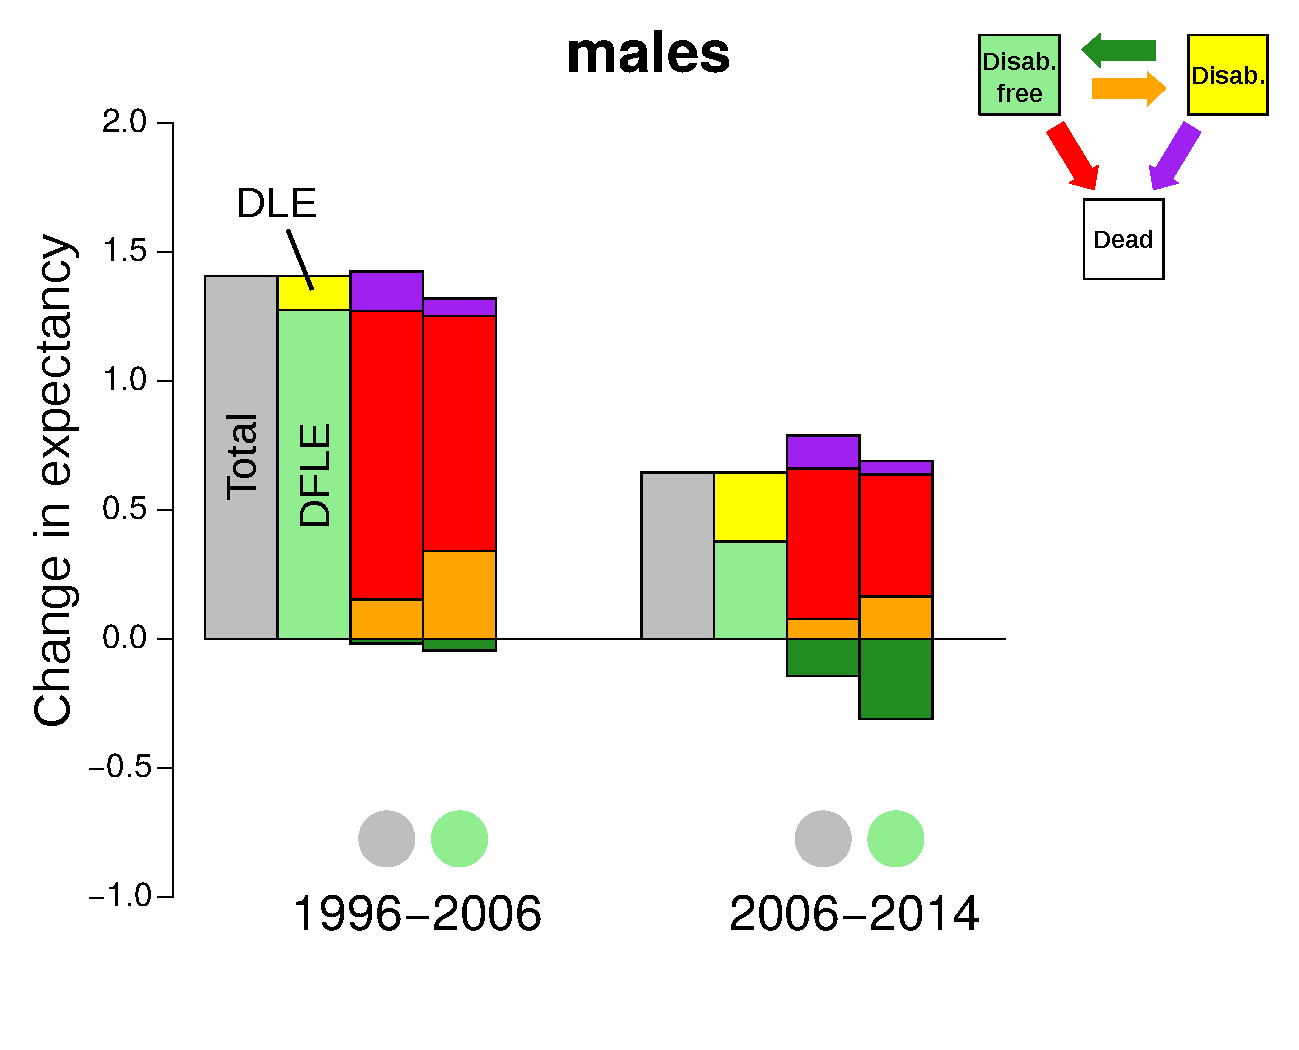
\includegraphics[height=\textheight, keepaspectratio]{Figures/MalesDecAllEdu4.pdf}}
%\only<5>{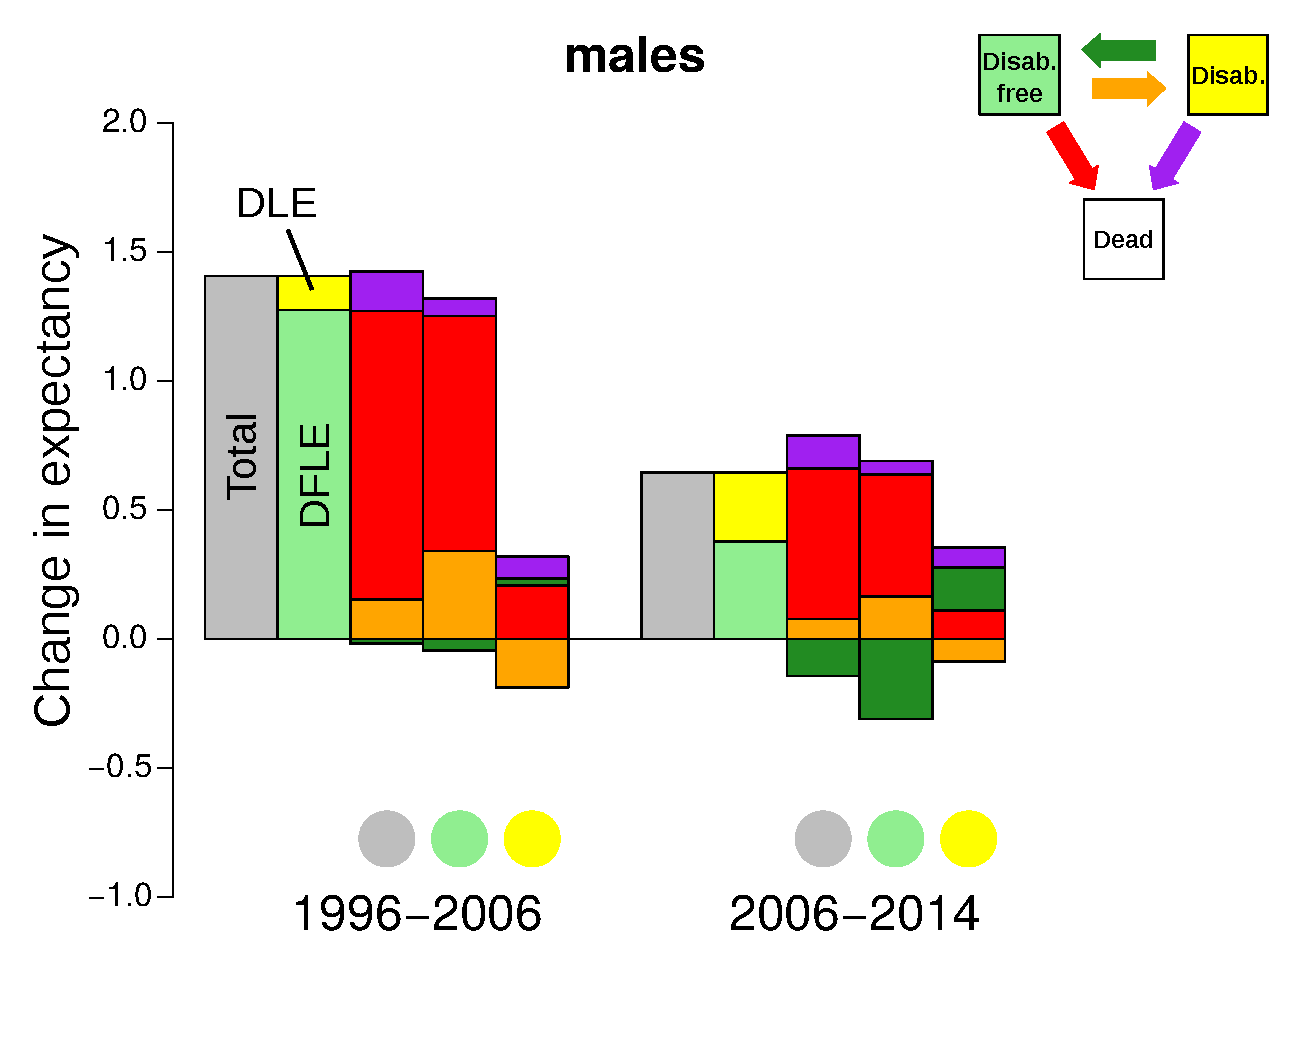
\includegraphics[height=\textheight, keepaspectratio]{Figures/MalesDecAllEdu5.pdf}}
%\only<6>{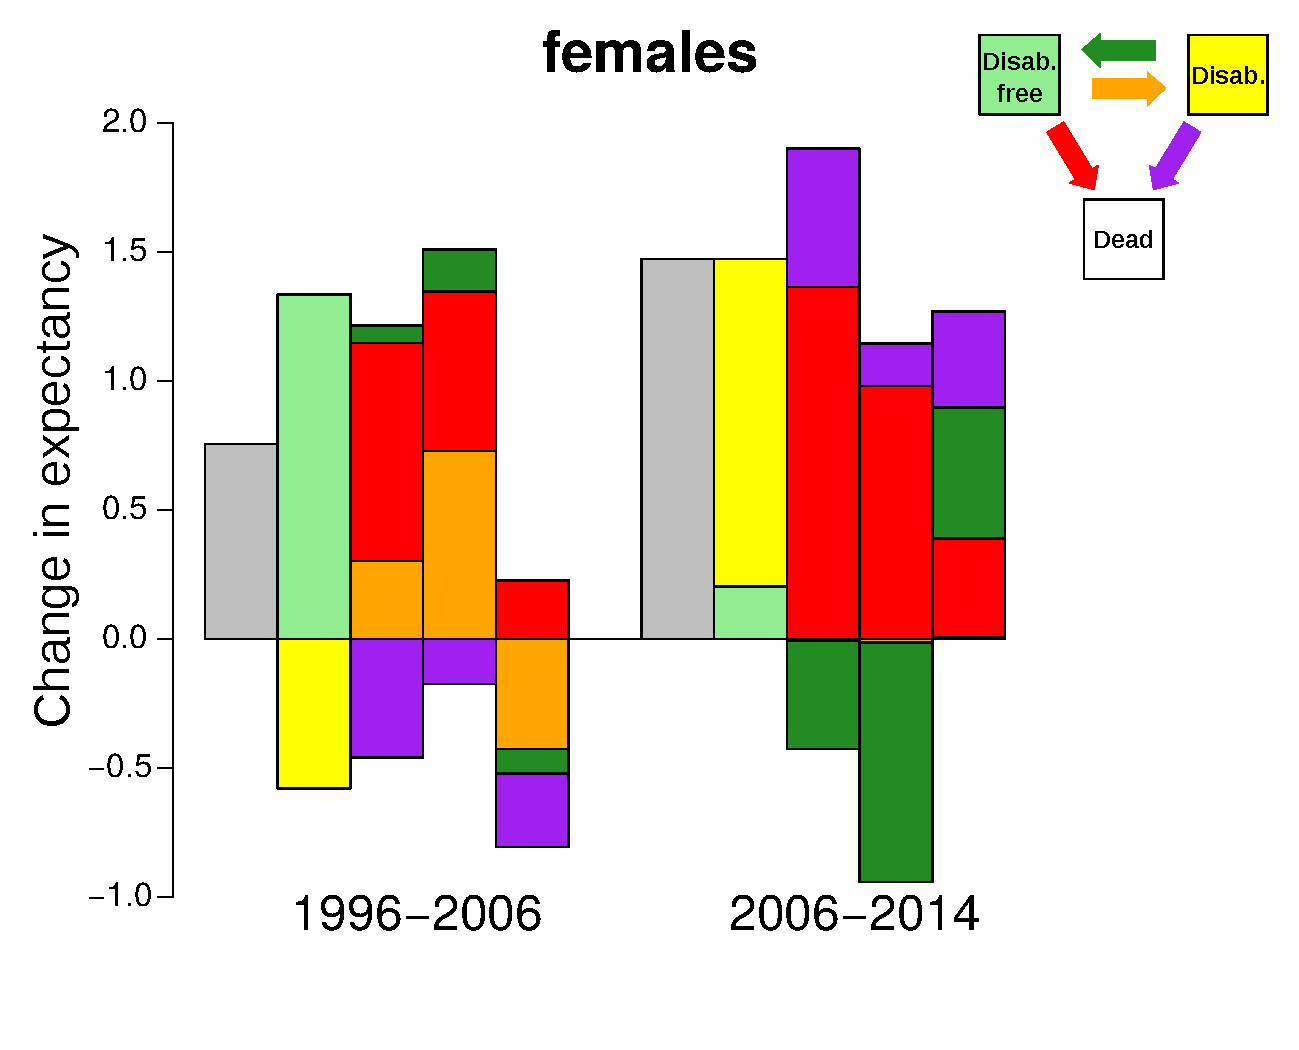
\includegraphics[height=\textheight, keepaspectratio]{Figures/FemalesDecAllEdu1.pdf}}
%\end{center}
%\end{overlayarea}
%\end{frame}
\begin{frame}[plain]
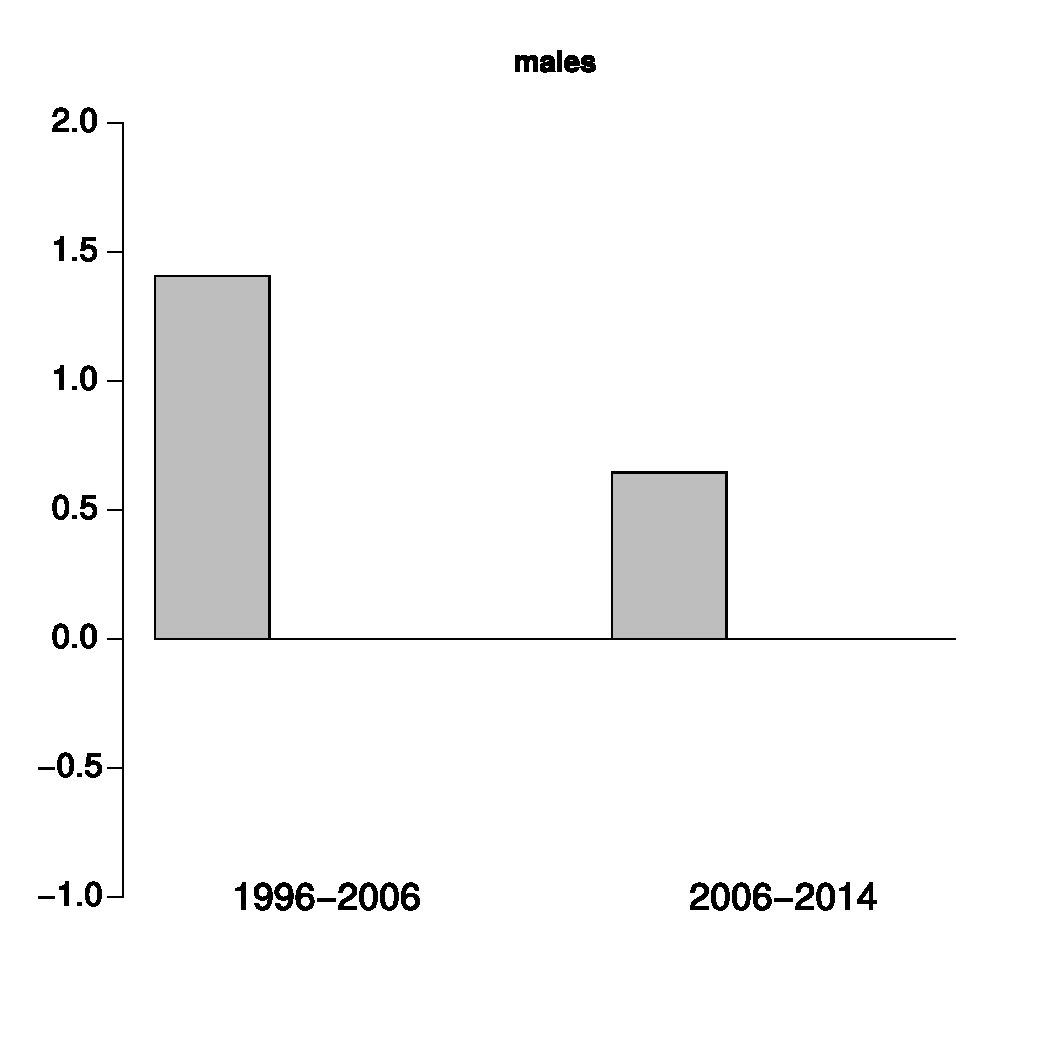
\includegraphics[height=\textheight, keepaspectratio]{Figures/MalesDecAllEdu1.pdf}
\end{frame}
\begin{frame}[plain]
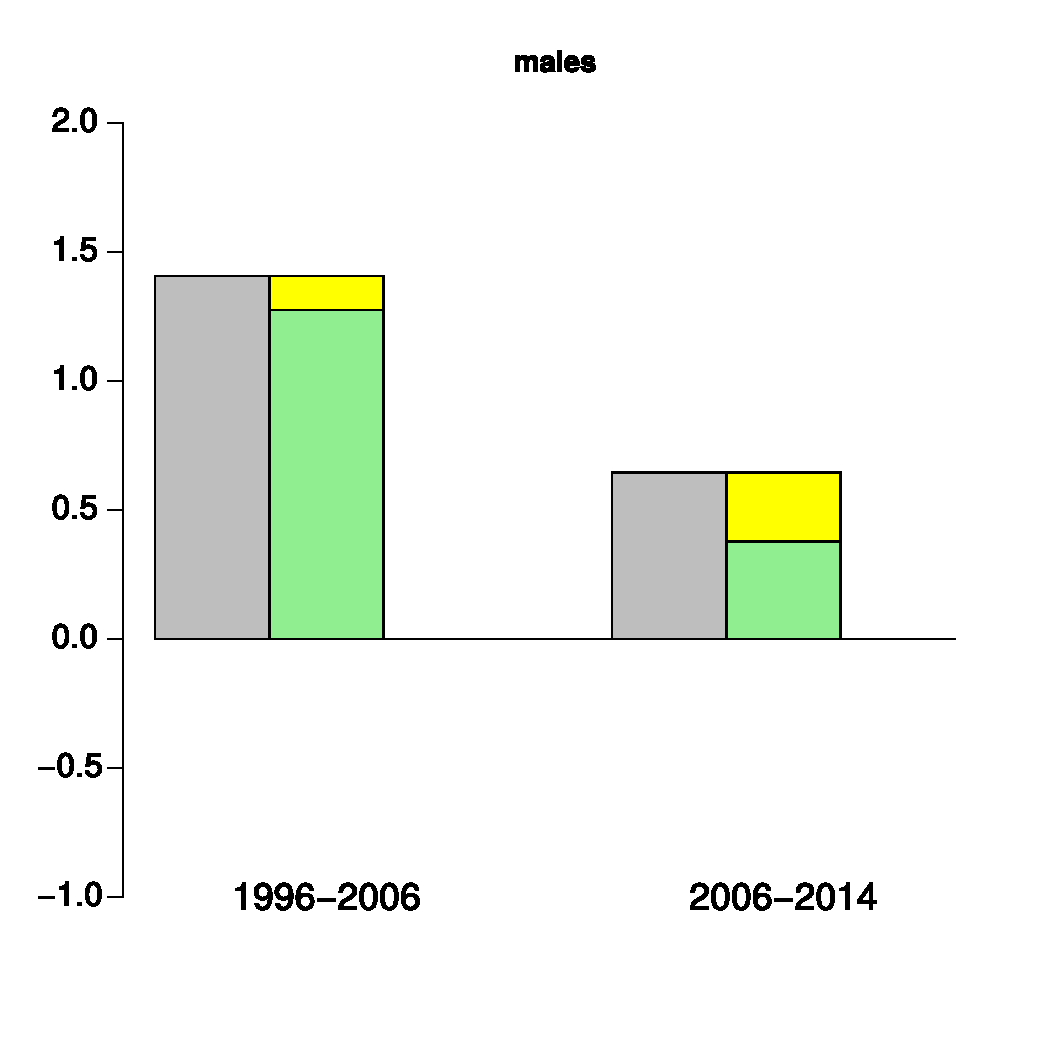
\includegraphics[height=\textheight, keepaspectratio]{Figures/MalesDecAllEdu2.pdf}
\end{frame}
\begin{frame}[plain]
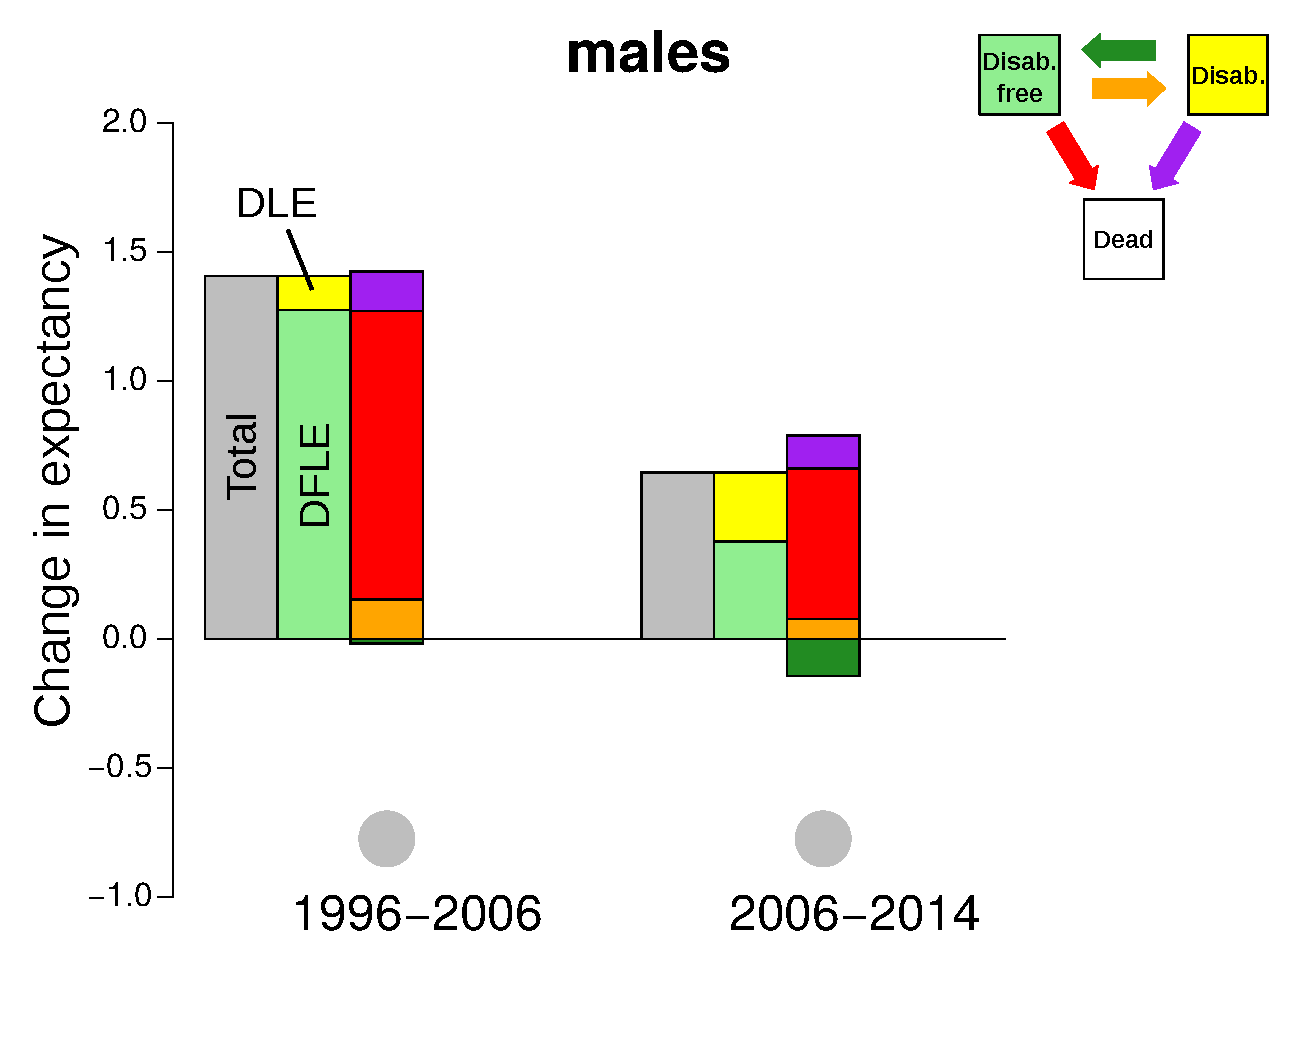
\includegraphics[height=\textheight, keepaspectratio]{Figures/MalesDecAllEdu3.pdf}
\end{frame}
\begin{frame}[plain]
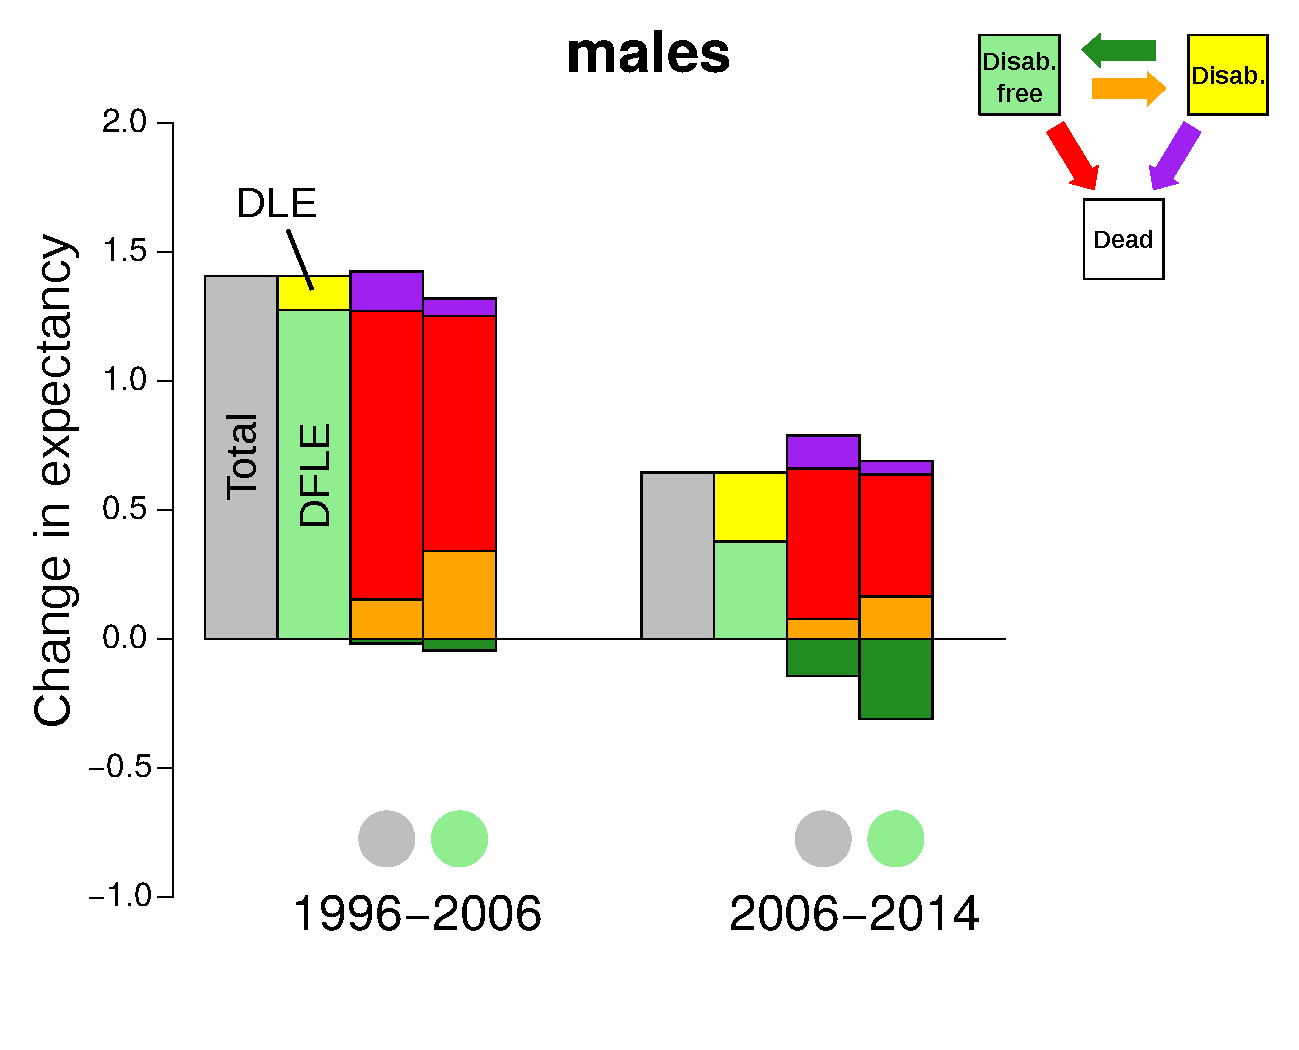
\includegraphics[height=\textheight, keepaspectratio]{Figures/MalesDecAllEdu4.pdf}
\end{frame}
\begin{frame}[plain]
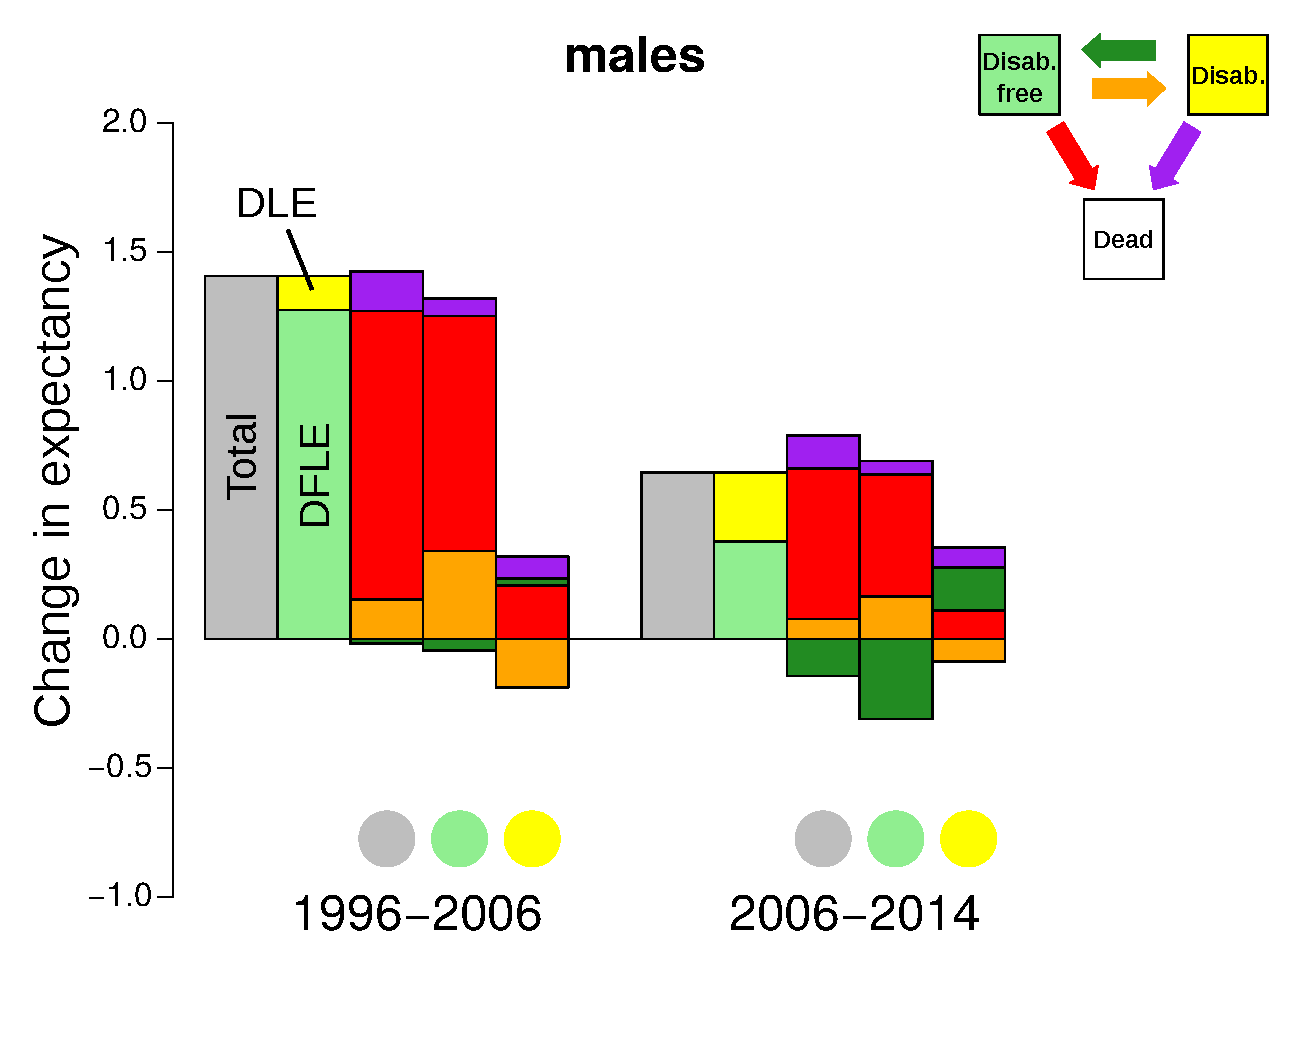
\includegraphics[height=\textheight, keepaspectratio]{Figures/MalesDecAllEdu5.pdf}
\end{frame}
\begin{frame}[plain]
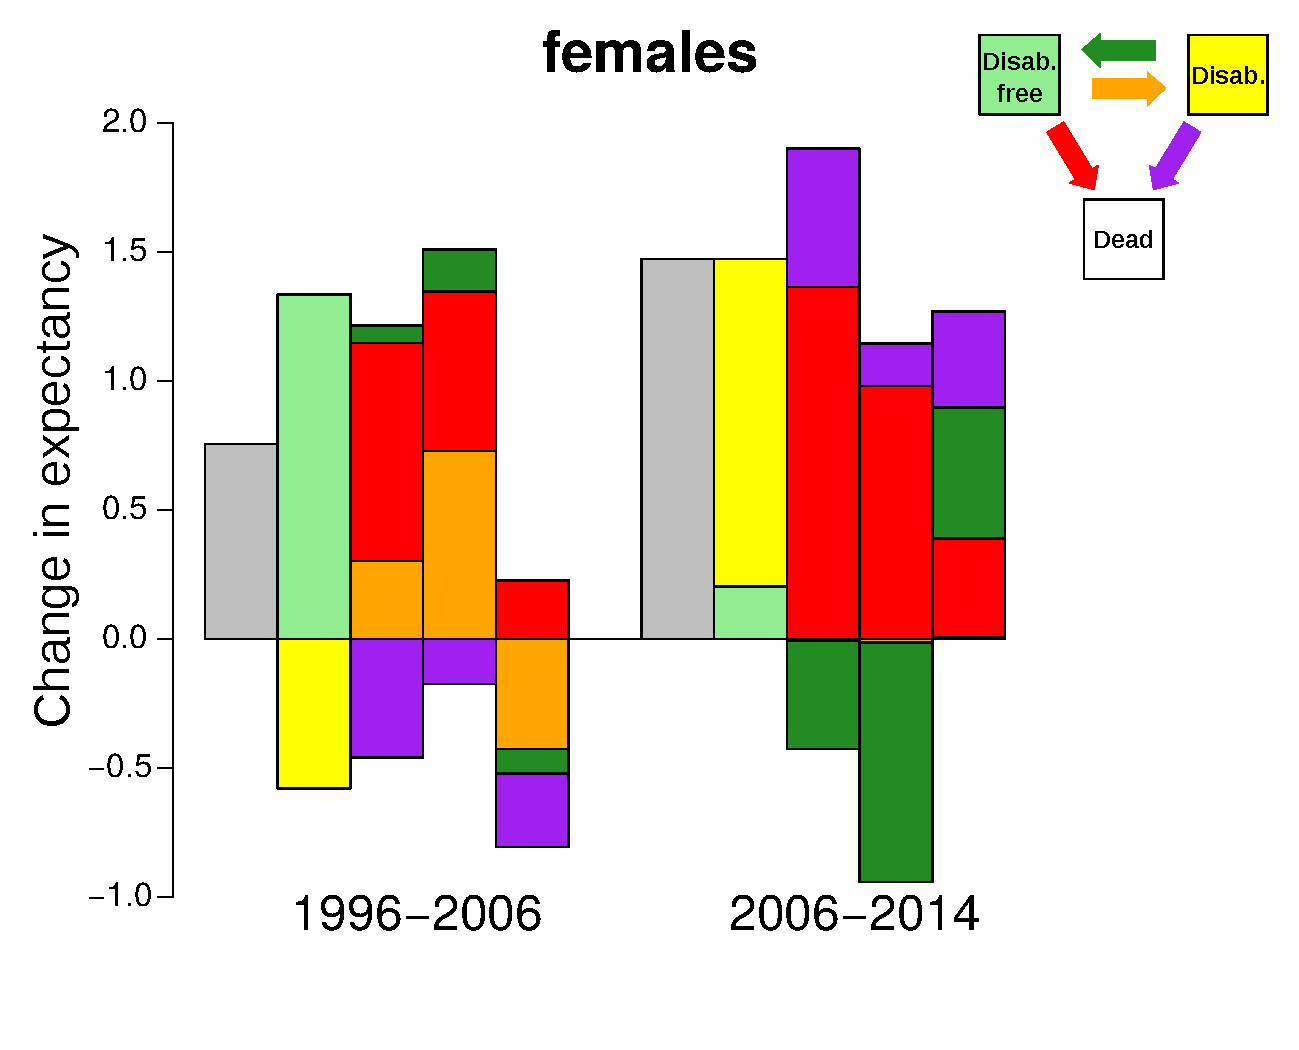
\includegraphics[height=\textheight, keepaspectratio]{Figures/FemalesDecAllEdu1.pdf}
\end{frame}


\begin{frame}[plain]
\Large
\begin{center}
Summary males:
\begin{itemize}[<+->]
\item most LE $\uparrow$ due to \textbf{DFLE $\uparrow$}.
\item \textbf{mortality improvement} 1996-2014 added 1.5 years to DFLE.
\item changes in transitions between disability and disability free largely \textbf{offset} one another.
\item DF \textbf{mortality change} always a \textbf{positive driver}.
\end{itemize}
\end{center}
\end{frame}

\begin{frame}[plain]
\Large
\begin{center}
Summary females:
\begin{itemize}[<+->]
\item \textbf{early} LE $\uparrow$ due to \textbf{DFLE $\uparrow$}, but reduced due to \textbf{lower DLE}.
\item most \textbf{early} DFLE $\uparrow$ due to \textbf{$\downarrow$ transitions to disability} and \textbf{$\uparrow$ recovery}.
\item \textbf{late} LE $\uparrow$ mostly due to \textbf{$\uparrow$ in DLE}.
\item itself mostly due to \textbf{$\downarrow$ mortality} and \textbf{$\downarrow$ recovery}.
\item early $\downarrow$ in transitions to disability \textbf{offset} by later $\downarrow$ in recovery.
\item DF \textbf{mortality change} always a \textbf{positive driver}.
\end{itemize}
\end{center}
\end{frame}

\begin{frame}[plain]
\Large
\begin{center}
\begin{itemize}[<+->]
\item Still some kinks with transition probability estimation.
\item Horiuchi decomposition works well with multistate models, other virtues.
\item So far only time decomps, other comparisons to come.
\item Mortality change major driver over time, but all transitions important.
\end{itemize}
\pause
Thanks!\\
riffe@demogr.mpg.de
\end{center}
\end{frame}


%%%%%%%%%%%%%%%%%%%%%%%%%%%%%%%%%%
%%	End of the document			%%
%%%%%%%%%%%%%%%%%%%%%%%%%%%%%%%%%%
\end{document}






